% !TEX root = /media/ueslei/Ueslei/INPE/PCI/Projetos/Guia_COAWST/main.tex
\chapterimage{header.jpg} % Chapter heading image

\chapter{COAWST in a parallel cluster}\index{COAWST na Kerana}
\bigskip

\section{About our cluster Kerana}
\bigskip

\noindent The CRAY XE machine, also called Kerana, is a cluster with massively parallel architecture, with 84 processing nodes and 2688 cores and is located at CPTEC/INPE,
in Cachoeira Paulista, São Paulo. For having the ability to parallelize operations through the MPI interface, the cluster is ideal for using numerical models with high spatial resolution
and temporal.
\bigskip

\section{Signing up a user account}
\bigskip

\noindent To start the process of applying for a user account in Kerana, it is necessary that the computer in the INPE's premises have a fixed IP. Your advisor or supervisor 
is required to send an email to \textit{Helpdesk} (\textcolor{bleu_cite}{\href{helpdesk.cptec@inpe.br}{\textit{helpdesk.cptec@inpe.br}}}) informing the MAC address, hostname
and reason for the request. If the computer already has a fixed IP assigned, it also need to be informed to be changed.
\bigskip

\noindent With the fixed IP configured, contact the \textit{Helpdesk} (\textcolor{bleu_cite}{\href{helpdesk.cptec@inpe.br}{\textit{helpdesk.cptec@inpe.br}}}) to request a form 
to use Kerana.
\bigskip

\section{Signing in to the Kerana cluster}\label{keranaacess}
\bigskip

\noindent Access will be done entirely through the computer terminal. You will need two primary commands: \textit{ssh} for accessing and manipulating files and folders and 
\textit{sftp} to download and upload files.
\bigskip

\noindent To access and modify files and folders, type in the terminal, replacing \textit{name.surname} with the user provided by \textit{Helpdesk}:
\bigskip

\begin{tcolorbox}[enhanced,
  grow to left by   = 0cm,
  grow to right by  = 0cm,
  enlarge top by    = 0cm,
  enlarge bottom by = 0cm,
  tcbox raise base,
  boxrule           = 1.0pt,
  left              = 18mm,
  colframe          = red!50!black,coltext=red!25!black,colback=red!10!white,
  overlay           = {\begin{tcbclipinterior}\fill[red!75!blue!50!white] (frame.south west)
    rectangle node[text=white,font=\sffamily\bfseries\footnotesize,rotate=0] {WARNING} ([xshift=18mm]frame.north west);\end{tcbclipinterior}}]
    From now on, whenever the guide shows the user as \textit{name.surname}, change to your username provided by the Helpdesk.
\end{tcolorbox}
\bigskip


\begin{bashcode}
ssh -Y name.surname@acesso-hpc.cptec.inpe.br -p 2000
\end{bashcode}
\bigskip

\noindent To download and/or upload, use:
\bigskip

\begin{bashcode}
sftp -P2000 name.surname@acesso-hpc.cptec.inpe.br
\end{bashcode}
\bigskip

\begin{tcolorbox}[enhanced,
  grow to left by   = 0cm,
  grow to right by  = 0cm,
  enlarge top by    = 0cm,
  enlarge bottom by = 0cm,
  tcbox raise base,
  boxrule           = 1.0pt,
  left              = 18mm,
  colframe          = red!50!black,coltext=red!25!black,colback=red!10!white,
  overlay           = {\begin{tcbclipinterior}\fill[red!75!blue!50!white] (frame.south west)
    rectangle node[text=white,font=\sffamily\bfseries\footnotesize,rotate=0] {WARNING} ([xshift=18mm]frame.north west);\end{tcbclipinterior}}]
It is not possible to download and upload multiple files at the same time using \textit{sftp}. One tip is to compress into a single \textit{tar} file and then unzip them.
\end{tcolorbox}
\bigskip

\noindent To add files from your computer to Kerana:
\bigskip

\begin{bashcode}
put file.tar.gz
\end{bashcode}
\bigskip

\noindent To extract Kerana files to your computer:
\bigskip

\begin{bashcode}
get file.tar.gz
\end{bashcode}
\bigskip

\section{File repository}\label{reposit}
\bigskip

\noindent Certain files are needed in each user's area to facilitate the use of the cluster. You will find them in the directory:
\bigskip

\begin{bashcode}
/scratch/adriano.sutil/repositorio/
\end{bashcode}
\bigskip

\noindent To copy the files to your area, type:
\bigskip

\begin{bashcode}
cp -r /scratch/adriano.sutil/repositorio /scratch/name.surname
\end{bashcode}
\bigskip

\begin{tcolorbox}[enhanced,
  grow to left by   = 0cm,
  grow to right by  = 0cm,
  enlarge top by    = 0cm,
  enlarge bottom by = 0cm,
  tcbox raise base,
  boxrule           = 1.0pt,
  left              = 18mm,
  colframe          = red!50!black,coltext=red!25!black,colback=red!10!white,
  overlay           = {\begin{tcbclipinterior}\fill[red!75!blue!50!white] (frame.south west)
    rectangle node[text=white,font=\sffamily\bfseries\footnotesize,rotate=0] {WARNING} ([xshift=18mm]frame.north west);\end{tcbclipinterior}}]
    From now on this guide will use the files that are inside this repository, so it is essential that they are in your area.
\end{tcolorbox}
\bigskip

\section{Kerana environment}
\bigskip

\noindent It is necessary to activate some modules in the cluster to compile COAWST. In this case, open the file \textit{.bashrc} which is located at the root directory of your user. 
\bigskip

\begin{bashcode}
vim .bashrc
\end{bashcode}
\bigskip

\noindent Add the following commands at the end of the file, changing only \textit{name.surname} to your username:
\bigskip


\begin{bashcode}
module load java
module load netcdf

export PATH=/scratch/name.surname/repositorio/Softs/nedit/5.5:$PATH
export PATH=/scratch/name.surname/repositorio/Softs/bin:$PATH

export PHDF5=${HDF_DIR}
export WRFIO_NCD_LARGE_FILE_SUPPORT=1

export PATH=/home/luciano.pezzi/local/bin:$PATH
export JASPERINC=/home/luciano.pezzi/local/include
export JASPERLIB=/home/luciano.pezzi/local/lib
export LD_LIBRARY_PATH=/home/luciano.pezzi/local/lib:$LD_LIBRARY_PATH
\end{bashcode}
\bigskip

\noindent Save and type in the terminal:
\bigskip

\begin{bashcode}
source .bashrc
\end{bashcode}

\section{Downloading COAWST}\label{coawstbaixa}
\bigskip

\begin{tcolorbox}[enhanced,
  grow to left by=0cm,%   equivalent to negative mdframed 'leftmargin'
  grow to right by=0cm,%  equivalent to negative mdframed 'rightmargin'
  enlarge top by=0cm,%     equivalent to mdframed 'skipabove'
  enlarge bottom by=0cm,%  equivalent to mdframed 'skipbelow'
  tcbox raise base,
  boxrule=1.0pt,
  left=18mm,
  colframe=red!50!black,coltext=red!25!black,colback=red!10!white,
  overlay={\begin{tcbclipinterior}\fill[red!75!blue!50!white] (frame.south west)
    rectangle node[text=white,font=\sffamily\bfseries\footnotesize,rotate=0] {WARNING} ([xshift=18mm]frame.north west);\end{tcbclipinterior}}]
COAWST v3.6 is already in the repository within the Kerana cluster, as discussed in Section \textcolor{bleu_cite}{\ref{reposit}}.
\end{tcolorbox}
\bigskip

\noindent To download COAWST, send an email to Dr. John Warner (\textcolor{bleu_cite}{\href{jcwarner@usgs.gov}{\textit{jcwarner@usgs.gov}}}), one of the heads behind the coupled regional modeling system.
\bigskip

\noindent After access is granted, with the user credentials and password provided by Dr. John Warner, type in the command the command below, changing the \ textit {myusrname} to your username.
\bigskip

\begin{bashcode}[fontsize=\footnotesize]
svn checkout --username myusrname https://coawstmodel.sourcerepo.com/coawstmodel/COAWST
\end{bashcode}
\bigskip

\noindent Add the COAWST folder to your Kerana desktop using \textit{sftp}, as in the Section \textcolor{bleu_cite}{\ref{keranaacess}}.
\bigskip

\section{Automating the compilation of COAWST in Kerana}\label{autowrf}
\bigskip

\begin{tcolorbox}[enhanced,
  grow to left by=0cm,%   equivalent to negative mdframed 'leftmargin'
  grow to right by=0cm,%  equivalent to negative mdframed 'rightmargin'
  enlarge top by=0cm,%     equivalent to mdframed 'skipabove'
  enlarge bottom by=0cm,%  equivalent to mdframed 'skipbelow'
  tcbox raise base,
  boxrule=1.0pt,
  left=18mm,
  colframe=red!50!black,coltext=red!25!black,colback=red!10!white,
  overlay={\begin{tcbclipinterior}\fill[red!75!blue!50!white] (frame.south west)
    rectangle node[text=white,font=\sffamily\bfseries\footnotesize,rotate=0] {WARNING} ([xshift=18mm]frame.north west);\end{tcbclipinterior}}]
  This guide uses COAWST v3.6.
\end{tcolorbox}
\bigskip

\noindent To speed up the process, it is possible to automate some compilation steps. Enter the directory:
\bigskip

\begin{bashcode}
cd /scratch/name.surname/COAWST/WRF/arch
\end{bashcode}
\bigskip

\noindent Open the file \textit{Config.pl}:
\bigskip

\begin{bashcode}
nedit Config.pl
\end{bashcode}
\bigskip

\noindent Look for the lines:
\bigskip

\begin{bashcode}[fontsize=\small]
printf "\nEnter selection [%d-%d] : ",1,$opt ;
$response = <STDIN> ;
\end{bashcode}
\bigskip

\noindent And replace \textit{<STDIN>} to 42, as in the example below:
\bigskip

\begin{bashcode}
printf "\nEnter selection [%d-%d] : ",1,$opt ;
$response = 42 ;
\end{bashcode}
\bigskip

\noindent Open the file \textit{configure.defaults}:
\bigskip

\begin{bashcode}
nedit configure.defaults
\end{bashcode}
\bigskip

\noindent Look for the \textit{TRADEFLAG}, option, which is on line 1262, approximately:
\bigskip

\begin{bashcode}
TRADEFLAG = CONFIGURE_TRADEFLAG
\end{bashcode}
\bigskip

\noindent And modify to:
\bigskip

\begin{bashcode}
TRADEFLAG = -traditional
\end{bashcode}
\bigskip

\noindent These modifications will select the configurations of the Kerana cluster (\textit{CRAY CCE (ftn/gcc): Cray XE and XC (dmpar)}), among those available to use COAWST, as shown in Figure \textcolor{bleu_cite}{\ref{compskerana}}.
\bigskip

\begin{figure}[H]
  \centering
  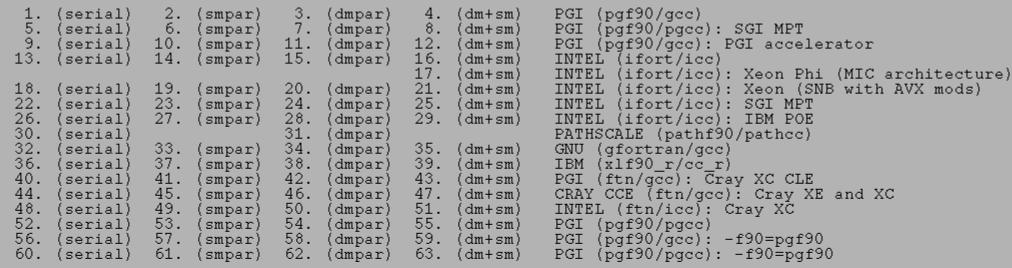
\includegraphics[width=0.80\textwidth]{linuxoptions.png}
  \caption{Computational options available for selection when compiling COAWST.}
  \label{compskerana}
\end{figure}
\bigskip

\noindent Now, in the same file, look for the following lines:
\bigskip

\begin{bashcode}[fontsize=\footnotesize]
printf "Compile for nesting? (1=basic, 2=preset moves, 3=vortex following) [default 1]: " ;
}
$response = <STDIN> ;
\end{bashcode}
\bigskip

\noindent And change \textit{<STDIN>} to the basic WRF atmospheric model nesting mode, as in the following example:
\bigskip

\begin{bashcode}[fontsize=\footnotesize]
printf "Compile for nesting? (1=basic, 2=preset moves, 3=vortex following) [default 1]: " ;
}
$response = 1 ;
\end{bashcode}
\bigskip

\section{Compiling the MCT}
\bigskip

\begin{tcolorbox}[enhanced,
  grow to left by=0cm,%   equivalent to negative mdframed 'leftmargin'
  grow to right by=0cm,%  equivalent to negative mdframed 'rightmargin'
  enlarge top by=0cm,%     equivalent to mdframed 'skipabove'
  enlarge bottom by=0cm,%  equivalent to mdframed 'skipbelow'
  tcbox raise base,
  boxrule=1.0pt,
  left=18mm,
  colframe=red!50!black,coltext=red!25!black,colback=red!10!white,
  overlay={\begin{tcbclipinterior}\fill[red!75!blue!50!white] (frame.south west)
    rectangle node[text=white,font=\sffamily\bfseries\footnotesize,rotate=0] {WARNING} ([xshift=18mm]frame.north west);\end{tcbclipinterior}}]
    This guide uses COAWST v 3.6.
\end{tcolorbox}
\bigskip


\noindent Each new user must compile the MCT before compiling COAWST. The first step is to use the \textit{setup\_pgi.sh} file. This file was copied from the previous 
repository, it is essential to change the directories contained therein. So open the file:
\bigskip

\begin{bashcode}
nedit setup_pgi.sh
\end{bashcode}
\bigskip

\noindent If necessary, change the directories according to the name of your COAWST folder and execute the file to load the necessary modules:
\bigskip

\begin{bashcode}
source setup_pgi.sh
\end{bashcode}
\bigskip

\noindent The libraries will be activated, as shown in Figure \textcolor{bleu_cite}{\ref{modulos}}:
\bigskip


\begin{figure}[H]
    \centering
    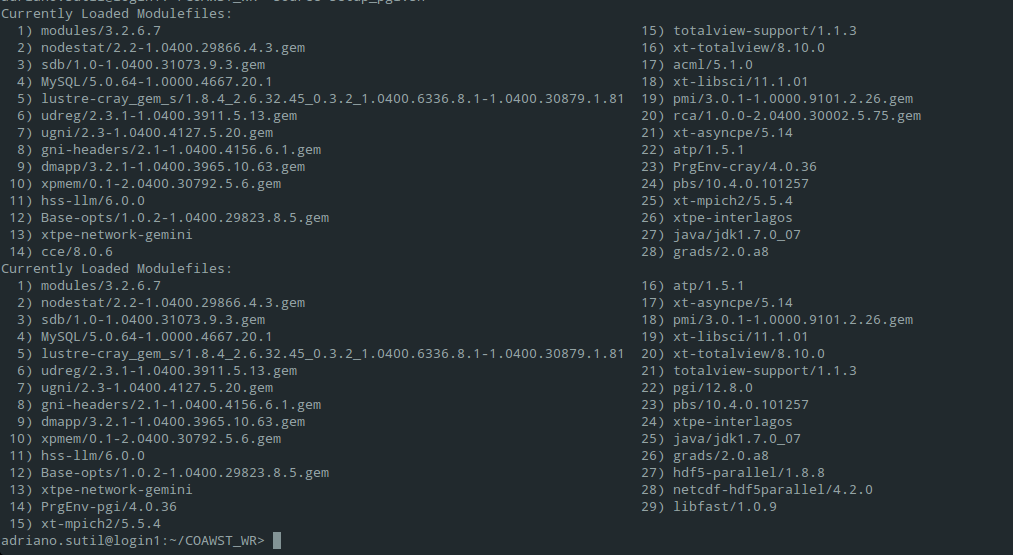
\includegraphics[width=0.85\textwidth]{modules.png}
    \caption{Modules activated in the cluster with the file \textit{setup\_pgi.sh} with user adriano.sutil.}
    \label{modulos}
\end{figure}
\bigskip

\noindent Enter the MCT folder directory:
\bigskip

\begin{bashcode}
cd /home/name.surname/COAWST/Lib/MCT
\end{bashcode}
\bigskip

\noindent Open the file \textit{Makefile.conf}:
\bigskip


\begin{bashcode}
nedit Makefile.conf
\end{bashcode}
\bigskip

\noindent And modify the file as follows:
\bigskip

\begin{tcolorbox}[enhanced,
  grow to left by=0cm,%   equivalent to negative mdframed 'leftmargin'
  grow to right by=0cm,%  equivalent to negative mdframed 'rightmargin'
  enlarge top by=0cm,%     equivalent to mdframed 'skipabove'
  enlarge bottom by=0cm,%  equivalent to mdframed 'skipbelow'
  tcbox raise base,
  boxrule=1.0pt,
  left=18mm,
  colframe=red!50!black,coltext=red!25!black,colback=red!10!white,
  overlay={\begin{tcbclipinterior}\fill[red!75!blue!50!white] (frame.south west)
    rectangle node[text=white,font=\sffamily\bfseries\footnotesize,rotate=0] {WARNING} ([xshift=18mm]frame.north west);\end{tcbclipinterior}}]
    Remember to change the \textit{name.surname}!
\end{tcolorbox}
\bigskip

\begin{bashcode}
FC  	    = ftn
FCFLAGS	 = -O2
F90FLAGS        = 
REAL8           = -r8
ENDIAN          = -Mbyteswapio
INCFLAG         = -I
INCPATH         =
MPILIBS         = 
DEFS            = -DSYSLINUX -DCPRPGI
FPP	     = cpp
FPPFLAGS        = -P -C -N -traditional
CC              = cc
ALLCFLAGS       = -DFORTRAN_UNDERSCORE_ -DSYSLINUX -DCPRPGI -O
COMPILER_ROOT   = 
BABELROOT       = 
PYTHON          = 
PYTHONOPTS      = 
FORT_SIZE       = 
CRULE           = .c.o
90RULE          = .F90.o
F90RULECPP      = .F90RULECPP
INSTALL         = /home/name.surname/COAWST/Lib/MCT/install-sh -c
MKINSTALLDIRS   = /home/name.surname/COAWST/Lib/MCT/mkinstalldirs
abs_top_builddir= /home/name.surname/COAWST/Lib/MCT/
MCTPATH         = /home/name.surname/COAWST/Lib/MCT/mct
MPEUPATH        = /home/name.surname/COAWST/Lib/MCT/mpeu
EXAMPLEPATH     = /home/name.surname/COAWST/Lib/MCT/examples
MPISERPATH      = 
libdir          = /home/name.surname/COAWST/Lib/MCT/pgi/lib
includedir      = /home/name.surname/COAWST/Lib/MCT/pgi/include
AR	      = ar cq
RM	      = rm -f
\end{bashcode}
\bigskip

\noindent Install the MCT by typing the following commands:
\bigskip

\begin{bashcode}
make
make install
\end{bashcode}
\bigskip
\noindent Observe the messages that appear in the terminal and look for errors. If not, the MCT was successfully compiled.
\bigskip


\section{Compiling the Sandy test case}
\bigskip

\noindent There are some test cases within COAWST to be compiled and worked on. In this case we’ll compile Hurricane Sandy’s project,
which couples and nests WRF, ROMS and SWAN. First, it is necessary to know the structure of COAWST files and folders.
\bigskip

\noindent The typical COAWST directory structure is exemplified in Figure \textcolor{bleu_cite}{\ref{pastascoa}}. Mainly, we will use the folders \textit{Projects} e \textit{Work} to work on.
\bigskip

\begin{figure}[H]
    \centering
    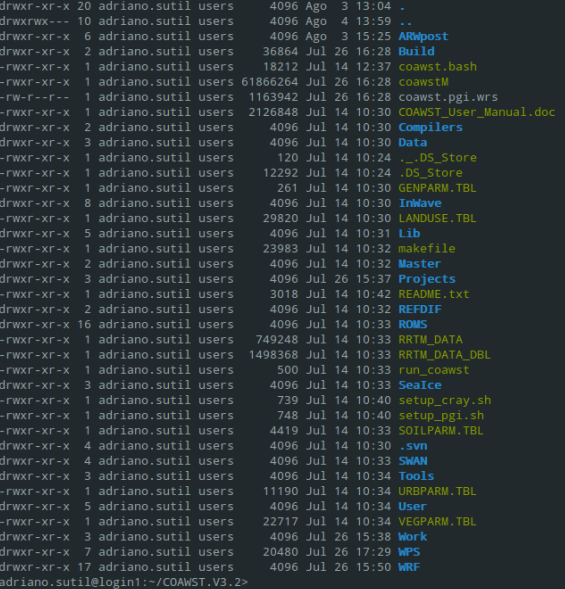
\includegraphics[width=0.50\textwidth]{estruturacoawst.png}
    \caption{
Representation of the main COAWST folder and subfolders.}
    \label{pastascoa}
\end{figure}
\bigskip

\subsection{Projects folder}\index{Pasta Projetcs}
\bigskip

\noindent To organize the projects, in the directory \textit{COAWST/Projects/Sandy} are all the files used to simulate the
Sandy case. The following files must be inside:
\bigskip

\begin{itemize}
\item Bound\_spec\_command
\item coastline.mat
\item coupling\_sandy.in
\item create\_sandy\_application.m
\item hycom\_info.mat
\item ijcoast.mat
\item multi\_1.at\_10m.dp.201210.grb2
\item multi\_1.at\_10m.hs.201210.grb2
\item multi\_1.at\_10m.tp.201210.grb2
\item namelist.input
\item ocean\_sandy.in
\item roms\_master\_climatology\_sandy.m
\item roms\_narr\_Oct2012.nc
\item roms\_narr\_ref3\_Oct2012.nc
\item Rweigths.txt
\item Sandy\_bdy.nc
\item Sandy\_clm.nc
\item Sandy\_clm\_ref3.nc
\item sandy.h
\item Sandy\_ini.nc
\item Sandy\_ini\_ref3.nc
\item Sandy\_init.hot
\item Sandy\_ref3\_init.hot
\item Sandy\_roms\_contact.nc
\item Sandy\_roms\_grid.nc
\item Sandy\_roms\_grid\_ref3.nc
\item Sandy\_swan\_bathy.bot
\item Sandy\_swan\_bathy\_ref3.bot
\item Sandy\_swan\_coord.grd
\item Sandy\_swan\_coord\_ref3.grd
\item scrip\_sandy\_moving.nc
\item scrip\_sandy\_static.nc
\item specpts.mat
\item swan\_narr\_Oct2012.dat
\item swan\_narr\_ref3\_Oct2012.dat
\item swan\_sandy.in
\item swan\_sandy\_ref3.in
\item tide\_forc\_Sandy.nc
\item TPAR10.txt
\item TPAR11.txt
\item TPAR12.txt
\item TPAR13.txt
\item TPAR14.txt
\item TPAR15.txt
\item TPAR16.txt
\item TPAR17.txt
\item TPAR18.txt
\item TPAR1.txt
\item TPAR2.txt
\item TPAR3.txt
\item TPAR4.txt
\item TPAR5.txt
\item TPAR6.txt
\item TPAR7.txt
\item TPAR8.txt
\item TPAR9.txt
\item USeast\_bathy.mat
\item Uweigths.txt
\item Vweigths.txt
\item wrfbdy\_d01
\item wrfinput\_d01
\item wrfinput\_d02
\item wrflowinp\_d01
\item wrflowinp\_d02
\end{itemize}
\bigskip

\subsection{Work folder}\index{Pasta Work}\label{workcoawstsec}
\bigskip

\noindent To make the management of simulations easier, it is suggested, for each new user, the creation of the \textit{Work} folder in
main COAWST directory, with each project inserted separately within it. It is in this folder that will be simulated
the test case.
\bigskip

\begin{bashcode}
cd /scratch/name.surname/COAWST
mkdir Work
cd Work
mkdir Sandy
\end{bashcode}
\bigskip

\noindent The folder \textit{/scratch/name.surname/COAWST/Work/Sandy} must contain the following files.
\bigskip

\begin{itemize}
\item run\_sandy.sh
\item limpa.sh
\item link.sh
\end{itemize}
\bigskip

\noindent The file \textit{run\_sandy.sh} will be used to start the simulation, \textit{link.sh} creates symbolic links in the folder \textit{Work}, 
that will be used by the models, and \textit{limpa.sh} is used to clear the folder if an error occurs and a new integration needs to be started. The files 
are inside the folder \textit{/repositorio/work\_coawst}.
\bigskip

\noindent Therefore:

\bigskip

\begin{bashcode}
cd /scratch/name.surname/repositorio/work_coawst
cp limpa.sh link.sh run_sandy.sh /scratch/name.surname/COAWST/Work/Sandy
\end{bashcode}
\bigskip

\noindent Go to the directory \textit{/scratch/name.surname/COAWST/Work/Sandy} and open the file\textit{run\_sandy.sh}:
\bigskip

\begin{bashcode}
cd /scratch/name.surname/COAWST/Work/Sandy
nedit run_sandy.sh
\end{bashcode}
\bigskip

\noindent Search for the following commands and modify the directories according to your username:
\bigskip

\begin{bashcode}
PBS -o /scratch/name.surname/COAWST/Work/Sandy/rws_total.out
ROOTDIR=/scratch/name.surname/COAWST
\end{bashcode}
\bigskip


\subsection{Compiling the test case}\index{Compilar o caso teste Sandy}
\bigskip

\noindent Go to the Sandy project folde:
\bigskip

\begin{bashcode}
/home/name.surname/COAWST/Projects/Sandy
\end{bashcode}
\bigskip

\noindent Open the following files to make changes to the next steps:
\bigskip

\begin{itemize}
\item coupling\_sandy.in
\item swan\_sandy.in
\item swan\_sandy\_ref3.in
\item ocean\_sandy.in
\end{itemize}
\bigskip

\begin{bashcode}
nedit coupling_sandy.in swan_sandy.in swan_sandy_ref3.in ocean_sandy.in
\end{bashcode}
\bigskip

\noindent Look for the command line below in the file \textit{coupling\_sandy.in}:
\bigskip

\begin{bashcode}
OCN_name = Projects/Sandy/ocean_sandy.in
\end{bashcode}
\bigskip

\noindent And replace with:
\bigskip

\begin{bashcode}
OCN_name = /scratch/name.surname/COAWST/Projects/Sandy/ocean_sandy.in
\end{bashcode}
\bigskip

\noindent In the files \textit{swan\_sandy.in} and \textit{swan\_sandy\_ref3.in} complete all directory paths below:
\bigskip

\noindent Modify:
\bigskip

\begin{bashcode}
READGRID COORDINATES 1 'Projects/Sandy/Sandy_swan_coord.grd' 4 0 0 FREE
READINP BOTTOM 1 'Projects/Sandy/Sandy_swan_bathy.bot' 4 0 FREE
&READINP WIND 1 'Projects/Sandy/swan_namnarr_30Sep10Nov2012.dat' 4 0 FREE
INITIAL HOTSTART SINGLE 'Projects/Sandy/Sandy_init.hot'
\end{bashcode}
\bigskip

\noindent By:
\bigskip

\begin{bashcode}[fontsize=\scriptsize]
READGRID COORDINATES 1 '/scratch/name.surname/COAWST/Projects/Sandy/Sandy_swan_coord.grd' 4 0 0 FREE
READINP BOTTOM 1 '/scratch/name.surname/COAWST/Projects/Sandy/Sandy_swan_bathy.bot' 4 0 FREE
&READINP WIND 1 '/scratch/name.surname/COAWST/Projects/Sandy/swan_namnarr_30Sep10Nov2012.dat' 4 0 FREE
INITIAL HOTSTART SINGLE '/scratch/name.surname/COAWST/Projects/Sandy/Sandy_init.hot'
\end{bashcode}
\bigskip

\noindent In the file \textit{ocean\_sandy.in} look for the command lines like below:
\bigskip

\begin{bashcode}
MyAppCPP = SANDY
VARNAME  = ROMS/External/varinfo.dat
GRDNAME == Projects/Sandy/Sandy_roms_grid.nc \
           Projects/Sandy/Sandy_roms_grid_ref3.nc
ININAME == Projects/Sandy/Sandy_ini.nc \
           Projects/Sandy/Sandy_ini_ref3.nc
NGCNAME =  Projects/Sandy/Sandy_roms_contact.nc
BRYNAME == Projects/Sandy/Sandy_bdy.nc
FRCNAME == Projects/Sandy/roms_narr_Oct2012.nc \
           Projects/Sandy/roms_narr_ref3_Oct2012.nc
\end{bashcode}
\bigskip

\noindent And replace with:
\bigskip

\begin{bashcode}[fontsize=\footnotesize]
MyAppCPP = Sandy
VARNAME  = /scratch/name.surname/COAWST/ROMS/External/varinfo.dat
GRDNAME == /scratch/name.surname/COAWST/Projects/Sandy/Sandy_roms_grid.nc \
           /scratch/name.surname/COAWST/Projects/Sandy/Sandy_roms_grid_ref3.nc
ININAME == /scratch/name.surname/COAWST/Projects/Sandy/Sandy_ini.nc \
           /scratch/name.surname/COAWST/Projects/Sandy/Sandy_ini_ref3.nc
NGCNAME =  /scratch/name.surname/COAWST/Projects/Sandy/Sandy_roms_contact.nc
BRYNAME == /scratch/name.surname/COAWST/Projects/Sandy/Sandy_bdy.nc
FRCNAME == /scratch/name.surname/COAWST/Projects/Sandy/roms_narr_Oct2012.nc \
           /scratch/name.surname/COAWST/Projects/Sandy/roms_narr_ref3_Oct2012.nc
\end{bashcode}
\bigskip

\noindent Go back to the main COAWST folder and open the file \textit{coawst.bash}:
\bigskip

\begin{bashcode}
cd /scratch/name.surname/COAWST
nedit coawst.bash
\end{bashcode}
\bigskip

\noindent Search for the following commands and modify, if necessary:
\bigskip

\begin{bashcode}
export   COAWST_APPLICATION=JOE_TC
export   MY_ROOT_DIR=${HOME}/COAWST
export   MY_HEADER_DIR=${MY_PROJECT_DIR}/Projects/JOE_TC
\end{bashcode}
\bigskip

\noindent By:
\bigskip

\begin{bashcode}
export   COAWST_APPLICATION=Sandy
export   MY_ROOT_DIR=${HOME}/COAWST
export   MY_HEADER_DIR=${MY_PROJECT_DIR}/Projects/Sandy
\end{bashcode}
\bigskip

\noindent Activate the modules again into the file \textit{setup\_pgi.sh}, and then compile the project with the command:
\bigskip

\begin{bashcode}
./coawst.bash -j 4  1> coawst.pgi.sandy 2>&1 &
\end{bashcode}
\bigskip

\noindent This command will create the text file \textit{coawst.pgi.sandy} where you can follow the progress of the compilation. Open the text file with the following 
command and look for the final message, as shown in Figure \textcolor{bleu_cite}{\ref{compcoafinal}}.
\bigskip

\begin{bashcode}
nedit coawst.pgi.sandy
\end{bashcode}
\bigskip

\begin{figure}[H]
    \centering
    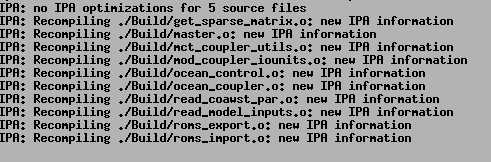
\includegraphics[width=0.65\textwidth]{coawstfinal.png}
    \caption{Final message after compiling COAWST.}
    \label{compcoafinal}
\end{figure}
\bigskip

\noindent If you want to follow the progress of the compilation through the terminal, use the command:
\bigskip

\begin{bashcode}
tail -f coawst.pgi.sandy
\end{bashcode}
\bigskip

\begin{tcolorbox}[enhanced,
  grow to left by=0cm,%   equivalent to negative mdframed 'leftmargin'
  grow to right by=0cm,%  equivalent to negative mdframed 'rightmargin'
  enlarge top by=0cm,%     equivalent to mdframed 'skipabove'
  enlarge bottom by=0cm,%  equivalent to mdframed 'skipbelow'
  tcbox raise base,
  boxrule=1.0pt,
  left=18mm,
  colframe=red!50!black,coltext=red!25!black,colback=red!10!white,
  overlay={\begin{tcbclipinterior}\fill[red!75!blue!50!white] (frame.south west)
    rectangle node[text=white,font=\sffamily\bfseries\footnotesize,rotate=0] {WARNING} ([xshift=18mm]frame.north west);\end{tcbclipinterior}}]
The compilation process is long!
\end{tcolorbox}
\bigskip


\noindent We finished! In the main COAWST directory, a file called \textit{coawstM} will be created. In this file all the information about your project 
will be compiled. Now with COAWST compiled, we will start the test case.
\bigskip

\section{Simulating the Sandy Test Case}\label{sandyexec}
\bigskip

\noindent To simulate the case, search for the \textit{run\_sandy.sh} file in \textit{Work/Sandy}. Type it:
\bigskip

\begin{bashcode}
cd /scratch/name.surname/COAWST/Work/Sandy
nedit run_sandy.sh
\end{bashcode}
\bigskip

\begin{tcolorbox}[enhanced,
  grow to left by=0cm,%   equivalent to negative mdframed 'leftmargin'
  grow to right by=0cm,%  equivalent to negative mdframed 'rightmargin'
  enlarge top by=0cm,%     equivalent to mdframed 'skipabove'
  enlarge bottom by=0cm,%  equivalent to mdframed 'skipbelow'
  tcbox raise base,
  boxrule=1.0pt,
  left=18mm,
  colframe=red!50!black,coltext=red!25!black,colback=red!10!white,
  overlay={\begin{tcbclipinterior}\fill[red!75!blue!50!white] (frame.south west)
    rectangle node[text=white,font=\sffamily\bfseries\footnotesize,rotate=0] {WARNING} ([xshift=18mm]frame.north west);\end{tcbclipinterior}}]
    The \textit{Work} folder should contain the files \textit{clean.sh}, \textit{link.sh} and \textit{run\_sandy.sh}. They can be found in the folder used as a repository. See Section \textcolor{bleu_cite} {\ref{workcoawstsec}}.
\end{tcolorbox}
\bigskip

\noindent When opening the file, check if the directories are in accordance with your username and type the command below to start the integration.
\bigskip

\begin{bashcode}
qsub run_sandy.sh
\end{bashcode}
\bigskip

\begin{tcolorbox}[enhanced,
  grow to left by=0cm,%   equivalent to negative mdframed 'leftmargin'
  grow to right by=0cm,%  equivalent to negative mdframed 'rightmargin'
  enlarge top by=0cm,%     equivalent to mdframed 'skipabove'
  enlarge bottom by=0cm,%  equivalent to mdframed 'skipbelow'
  tcbox raise base,
  boxrule=1.0pt,
  left=18mm,
  colframe=red!50!black,coltext=red!25!black,colback=red!10!white,
  overlay={\begin{tcbclipinterior}\fill[red!75!blue!50!white] (frame.south west)
    rectangle node[text=white,font=\sffamily\bfseries\footnotesize,rotate=0] {WARNING} ([xshift=18mm]frame.north west);\end{tcbclipinterior}}]
 The command \textit{qsub} will submit you job. It will send the executed script to a batch of the cluster, reserving a part of the processors for your simulation.
\end{tcolorbox}
\bigskip

\noindent The process will generate two files to follow the evolution of the simulation: \textit{log.out} and \textit{log.err}. To open, use:
\bigskip

\begin{bashcode}
nedit log.out log.err
\end{bashcode}
\bigskip

\noindent Or look directly at the terminal with the command:
\bigskip

\begin{bashcode}
tail -f log.out
\end{bashcode}
\bigskip

\noindent The outputs of the simulations will be stored in the \textit{Work/Sandy} folder. If an error occurs, clean the desktop with the command:
\bigskip

\begin{bashcode}
./limpa.sh
\end{bashcode}
\bigskip


\begin{tcolorbox}[enhanced,
  grow to left by=0cm,%   equivalent to negative mdframed 'leftmargin'
  grow to right by=0cm,%  equivalent to negative mdframed 'rightmargin'
  enlarge top by=0cm,%     equivalent to mdframed 'skipabove'
  enlarge bottom by=0cm,%  equivalent to mdframed 'skipbelow'
  tcbox raise base,
  boxrule=1.0pt,
  left=18mm,
  colframe=red!50!black,coltext=red!25!black,colback=red!10!white,
  overlay={\begin{tcbclipinterior}\fill[red!75!blue!50!white] (frame.south west)
    rectangle node[text=white,font=\sffamily\bfseries\footnotesize,rotate=0] {WARNING} ([xshift=18mm]frame.north west);\end{tcbclipinterior}}]
    The simulation of the may take several hours when integrating using 3 processors.
\end{tcolorbox}
\bigskip
